\section{Evaluating Effects of Barium Sulfate\label{sec:methodology:effectsOfBaSO4}}

The effects of barium sulfate concentration (imaging and mechanical properties) when incorporated with PLA were analyzed. The goal of this analysis was to determine the optimal barium sulfate concentration required for imaging, and ensure the material properties at this concentration were within usable ranges for this implantable device.

\subsection{Imaging Study\label{sec:methodology:effectsOfBaSO4:imagingStudy}}

A predominant goal of the barium sulfate extrusions and printing was to evaluate its effects on radiopacity. To measure these effects, an imaging study was conducted. This study was conducted in collaboration with the Stephanie Spielman Comprehensive Breast Center (OSUCCC).

\subsubsection{Sample Preparation\label{sec:methodology:effectsOfBaSO4:imagingStudy:samplePrep}}

Samples were prepared based on similar conducted literature~\cite{RefWorks:RefID:77-hamedani2018threedimensional}. A $1cm$ wide and $1cm$ tall cylinder was designed in SolidWorks, and numerous samples were printed for each barium sulfate concentration group. Based on limited supply of extruded filament, four samples were printed for each concentration group.

To minimize air gaps, samples were printed with 100\% infill.

The various 3D printed samples for imaging are shown below in Figure~\ref{fig:methodology:effectsOfBaSO4:imagingStudySamples}

\begin{figure}[h!]
        \centering
        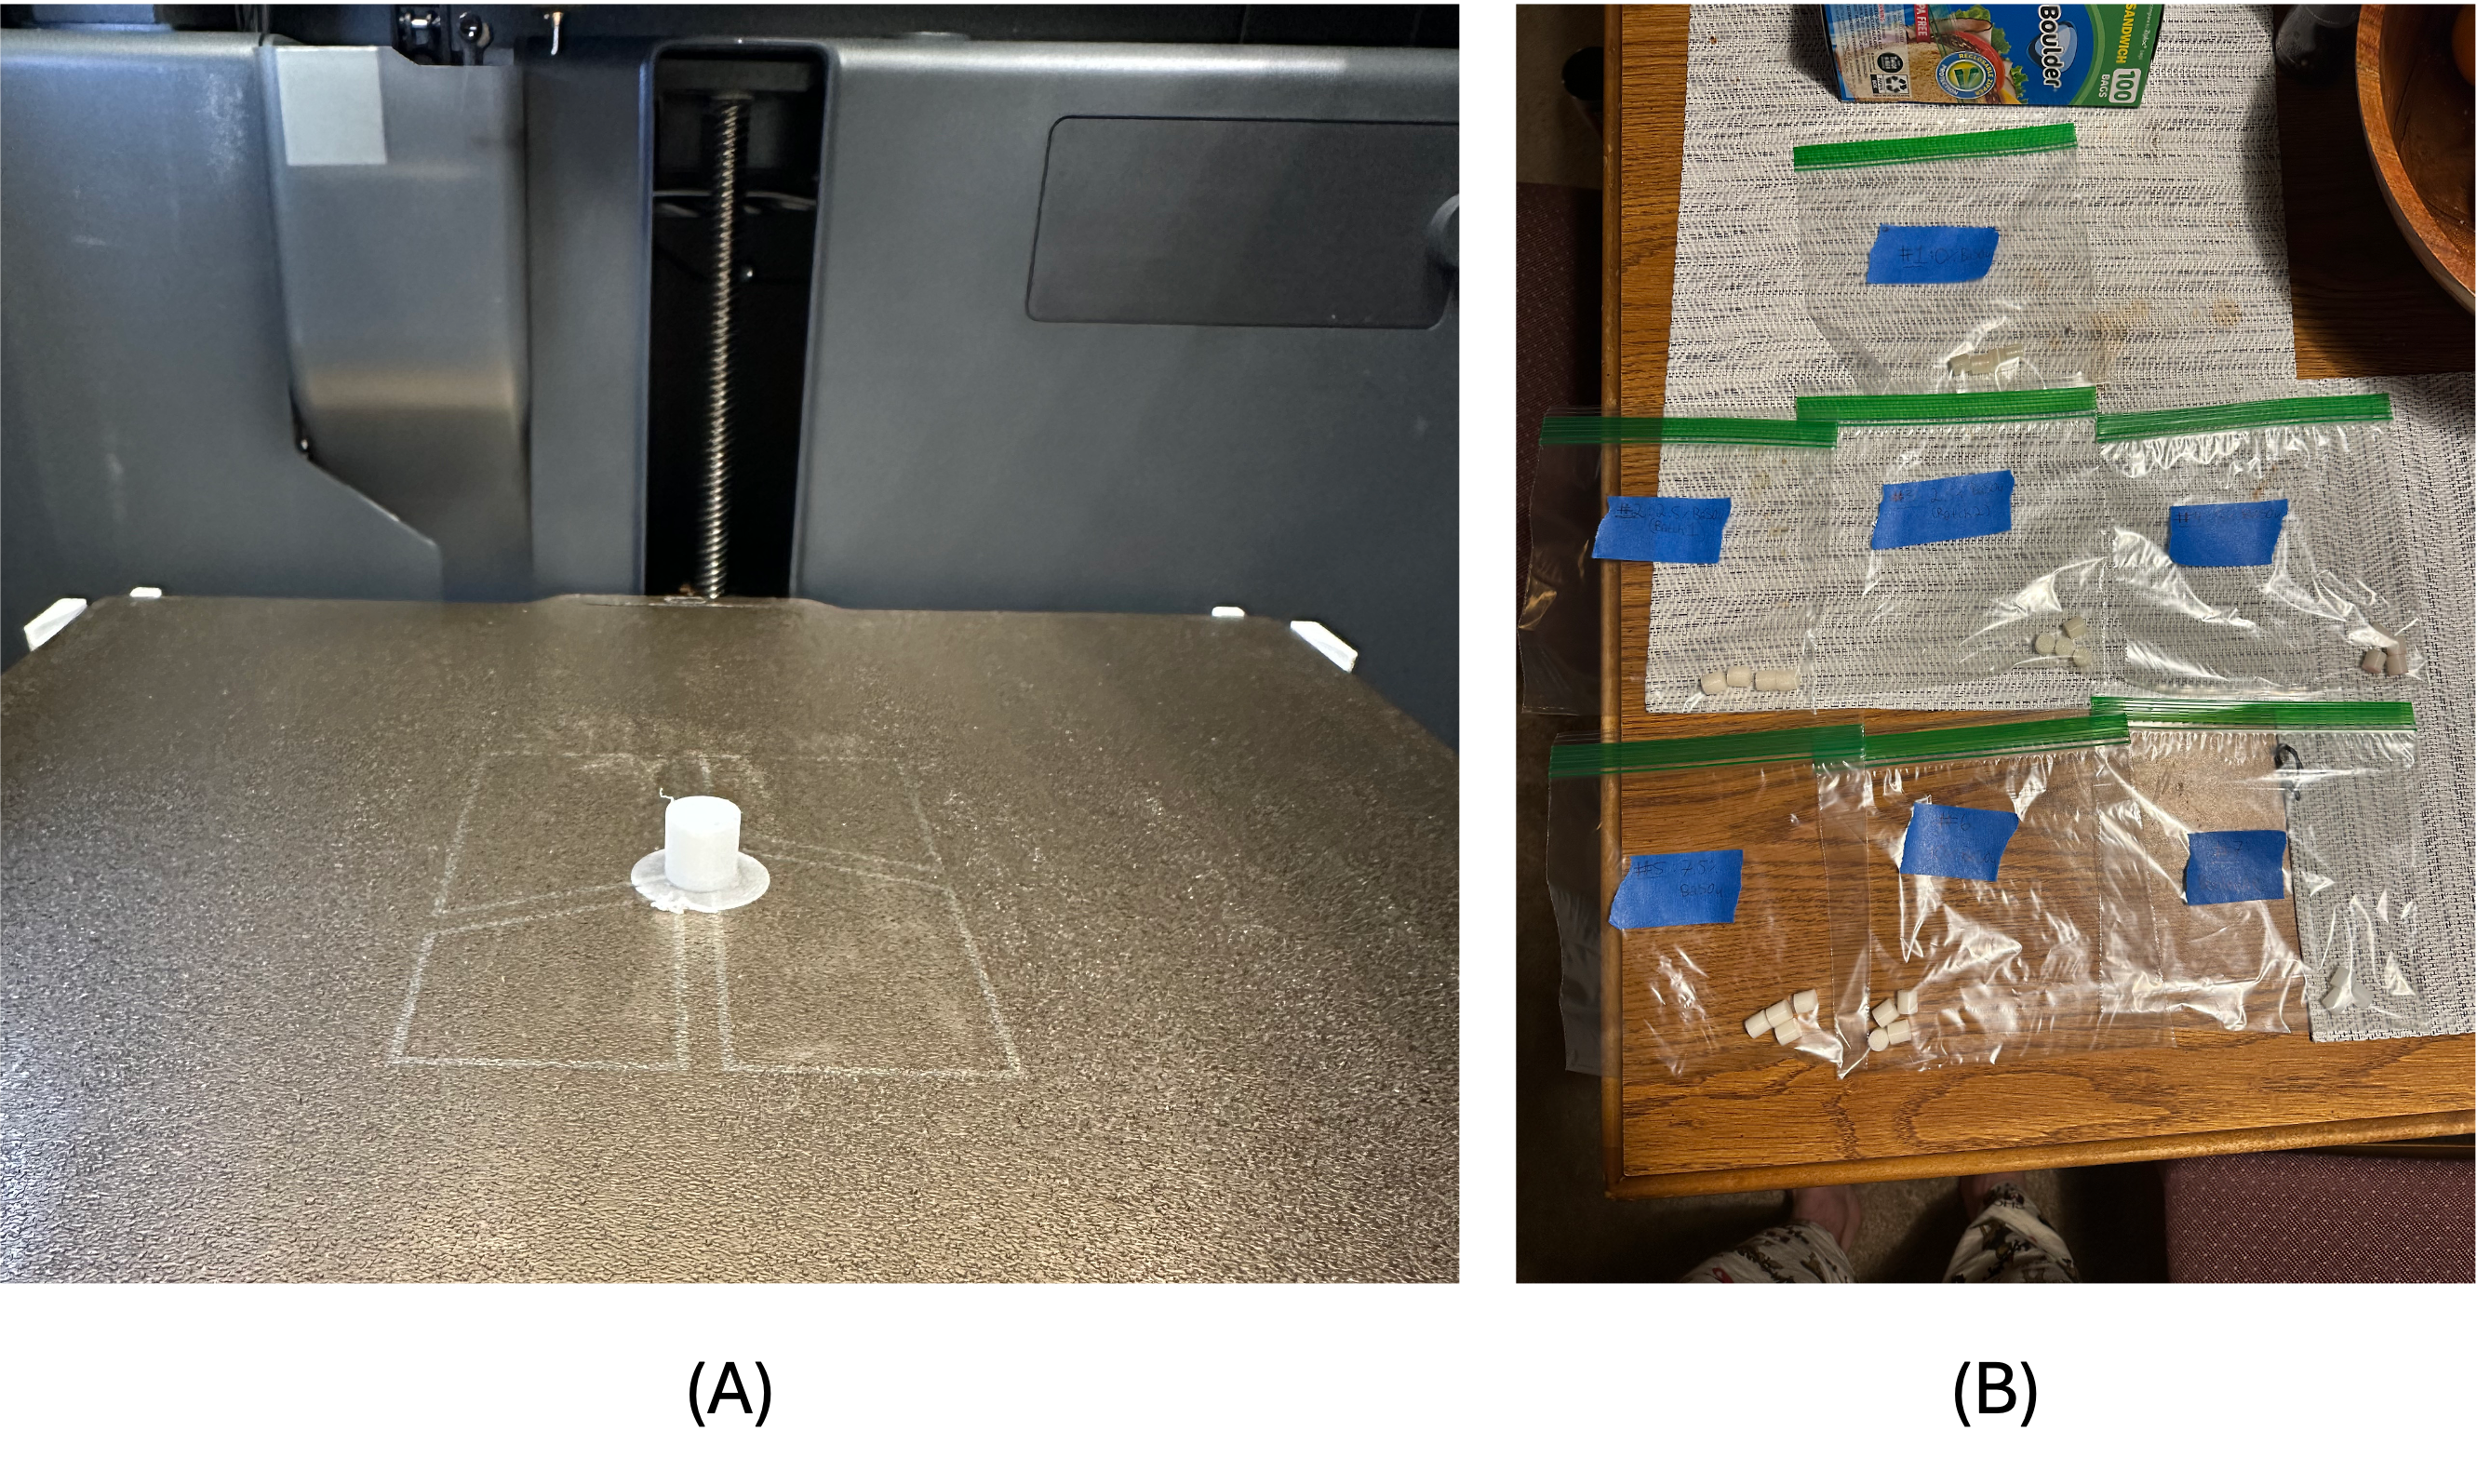
\includegraphics[width=\linewidth]{../figs/methodology/imagingStudy/imaging_study_samples.png}
        \caption{Imaging study samples. Individual printed sample (A) and all final bagged samples (B).}
        \label{fig:methodology:effectsOfBaSO4:imagingStudySamples}
\end{figure}

\subsubsection{Bonlecule Filament\label{sec:methodology:effectsOfBaSO4:imagingStudy:bonlecule}}

In addition to the custom-made PLA/BaSO\textsubscript{4} filaments, a commercially made radiopaque filament, Bonlecule, was also tested. A sample of this filament was sent from NOVUS~\cite{RefWorks:RefID:78-bonlecule}.

To 3D print Bonlecule, printing parameters from the manufacturer were used based initially on PLA Marble presets. Table~\ref{tab:methodology:bonleculeParameters} summarizes the final printing parameters used for this filament. Additionally, following manufacturer suggestions, glue was applied to the build plate to improve build plate adhesion.

Due to limited filament initially supplied, three samples of Bonlecule filament rather than four were printed for this imaging study.

\begin{table}[h!]
        \centering
        \caption{Printing parameters for Bonlecule filament.}
        \label{tab:methodology:bonleculeParameters}
        \begin{tabular}{l l}
                \hline
                \textbf{Parameter}               & \textbf{Value}    \\
                \hline
                Base Material                    & Unknown           \\
                Vendor / Extruder                & Bonlecule         \\
                Initial Preset                   & PLA Marble        \\
                BaSO$_4$ \%                      & Unknown           \\
                Nozzle Size (mm)                 & 0.6 Cold Hardened \\
                Initial Layer                    & 35                \\
                Initial Layer Infill             & 55                \\
                Outer Wall                       & 120               \\
                Inner Wall                       & 150               \\
                Sparse Infill                    & 120               \\
                Internal Solid Infill            & 150               \\
                Recommended Nozzle Temp Range    & 220--240          \\
                Textured PEI Plate Initial Layer & 85                \\
                Textured PEI Plate Other Layers  & 85                \\
                Nozzle Initial Layer             & 230               \\
                Nozzle Other Layers              & 230               \\
                Max Volumetric Speed (mm$^3$/s)  & 8                 \\
                \hline
        \end{tabular}
\end{table}


Samples were given to OSUCCC where Dr. Eric Cochran helped image all samples.

Results and discussion of this imaging study can be found in~\fullref{sec:results:effectsOfBaSO4:imagingStudy} and~\fullref{sec:discussion:effectsOfBaSO4:imagingStudy} respectively.

\subsection{Tensile Testing\label{sec:methodology:effectsOfBaSO4:tensileTesting}}

Tensile testing was performed with the PLA/BaSO\textsubscript{4} samples to determine how concentrations of barium sulfate impact the yield strength and elastic modulus of a material. These properties indicate the extent of plastic deformation a material can withstand and will help determine the maximum allowable amount of barium sulfate in the implant based on how it impacts material properties.

All tensile testing was performed on an Instron 5859 Universal Testing System at the Center for Design and Manufacturing Excellence (CDME) at The Ohio State University.

\subsubsection{Sample Preparation\label{sec:methodology:effectsOfBaSO4:tensileTesting:samplePrep}}

Following ASTM D638 testing standard for tensile testing, there are five test specimen geometries that can be used. Type I is the recommended specimen, but Type V is recommended when material is limited. This is explored further in~\fullref{sec:literatureReview:testing:specimens}.

Due to limited 3D printable filament and the time involved in extruding more PLA/BaSO\textsubscript{4} filament samples, Type V test specimen were initially 3D printed to preserve material. A 100\% infill density was used to most closely match the material properties of the raw material (see~\fullref{sec:literatureReview:printing:optimalParameters:infillDensity}).

Once 3D printed, samples were measured following ASTM D638 test standard and marked for testing. An example of the marked samples are shown below in Figure~\ref{fig:methodology:effectsofBaSO4:tensileTest:samplePrep}.

\begin{figure}[h!]
        \centering
        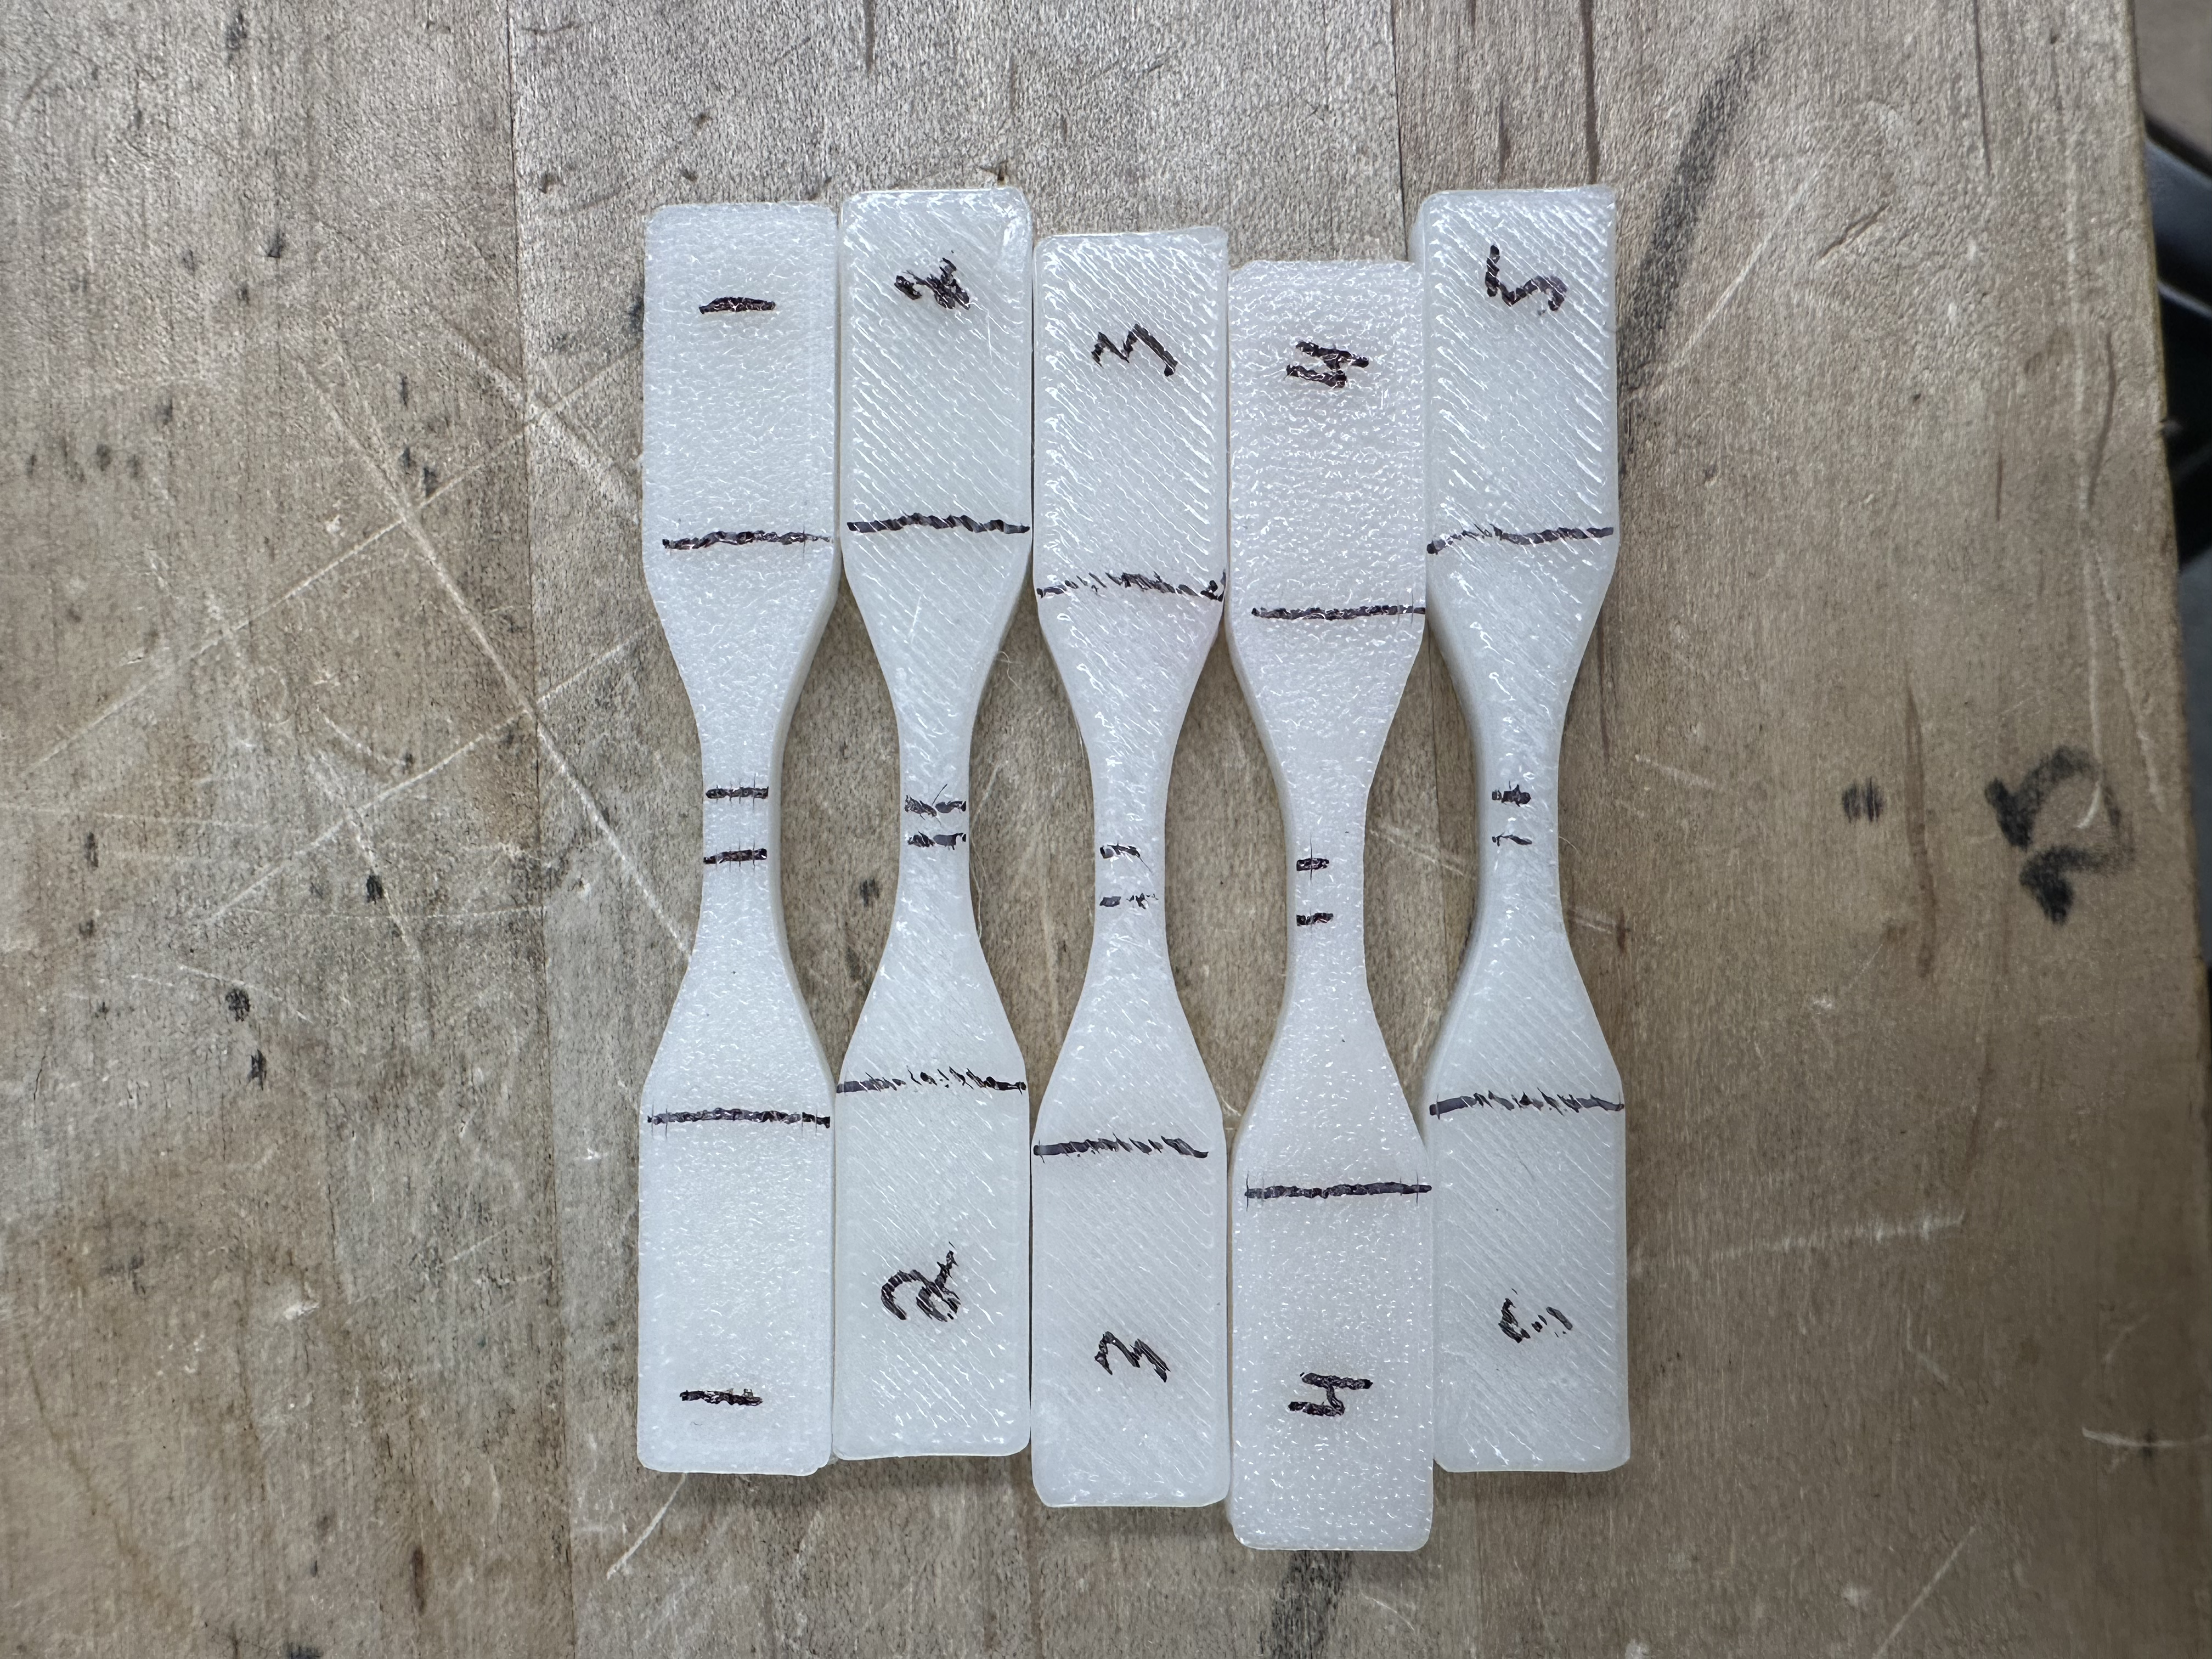
\includegraphics[width=0.5\linewidth]{../figs/methodology/mechanicalTesting/tensileTesting/tensile_test_marked_samples.png}
        \caption{Marked samples in preparation of tensile testing.}
        \label{fig:methodology:effectsofBaSO4:tensileTest:samplePrep}
\end{figure}

Cross-sectional area was calculated based on the average measured width and thickness of the rectangular gage length of the test specimen. For both width and thickness, the average of three measurements was recorded. The cross-sectional area of the test specimen is illustrated below in Figure~\ref{methodology:effectsofBaSO4:tensileTest:crossSectionalArea}.

\begin{figure}[h!]
        \centering
        \includegraphics[width=0.5\linewidth]{../figs/methodology/mechanicalTesting/tensileTesting/cross_sectional_area.png}
        \caption{Cross sectional area of test specimen~\cite{RefWorks:RefID:370-einsteinisaac}.}
        \label{methodology:effectsofBaSO4:tensileTest:crossSectionalArea}
\end{figure}

\subsubsection{Performing Tensile Tests\label{sec:methodology:effectsOfBaSO4:tensileTesting:performingTest}}

After measurements were recorded, samples were loaded into an Instron 5859 Universal Testing System as shown in Figure~\ref{fig:methodology:effectsofBaSO4:tensileTest:loadingSamples}. A pre-build ASTM D638 tensile test method was utilized to perform the test. Results were calculated automatically through the Instron software and recorded locally.

\begin{figure}[h!]
        \centering
        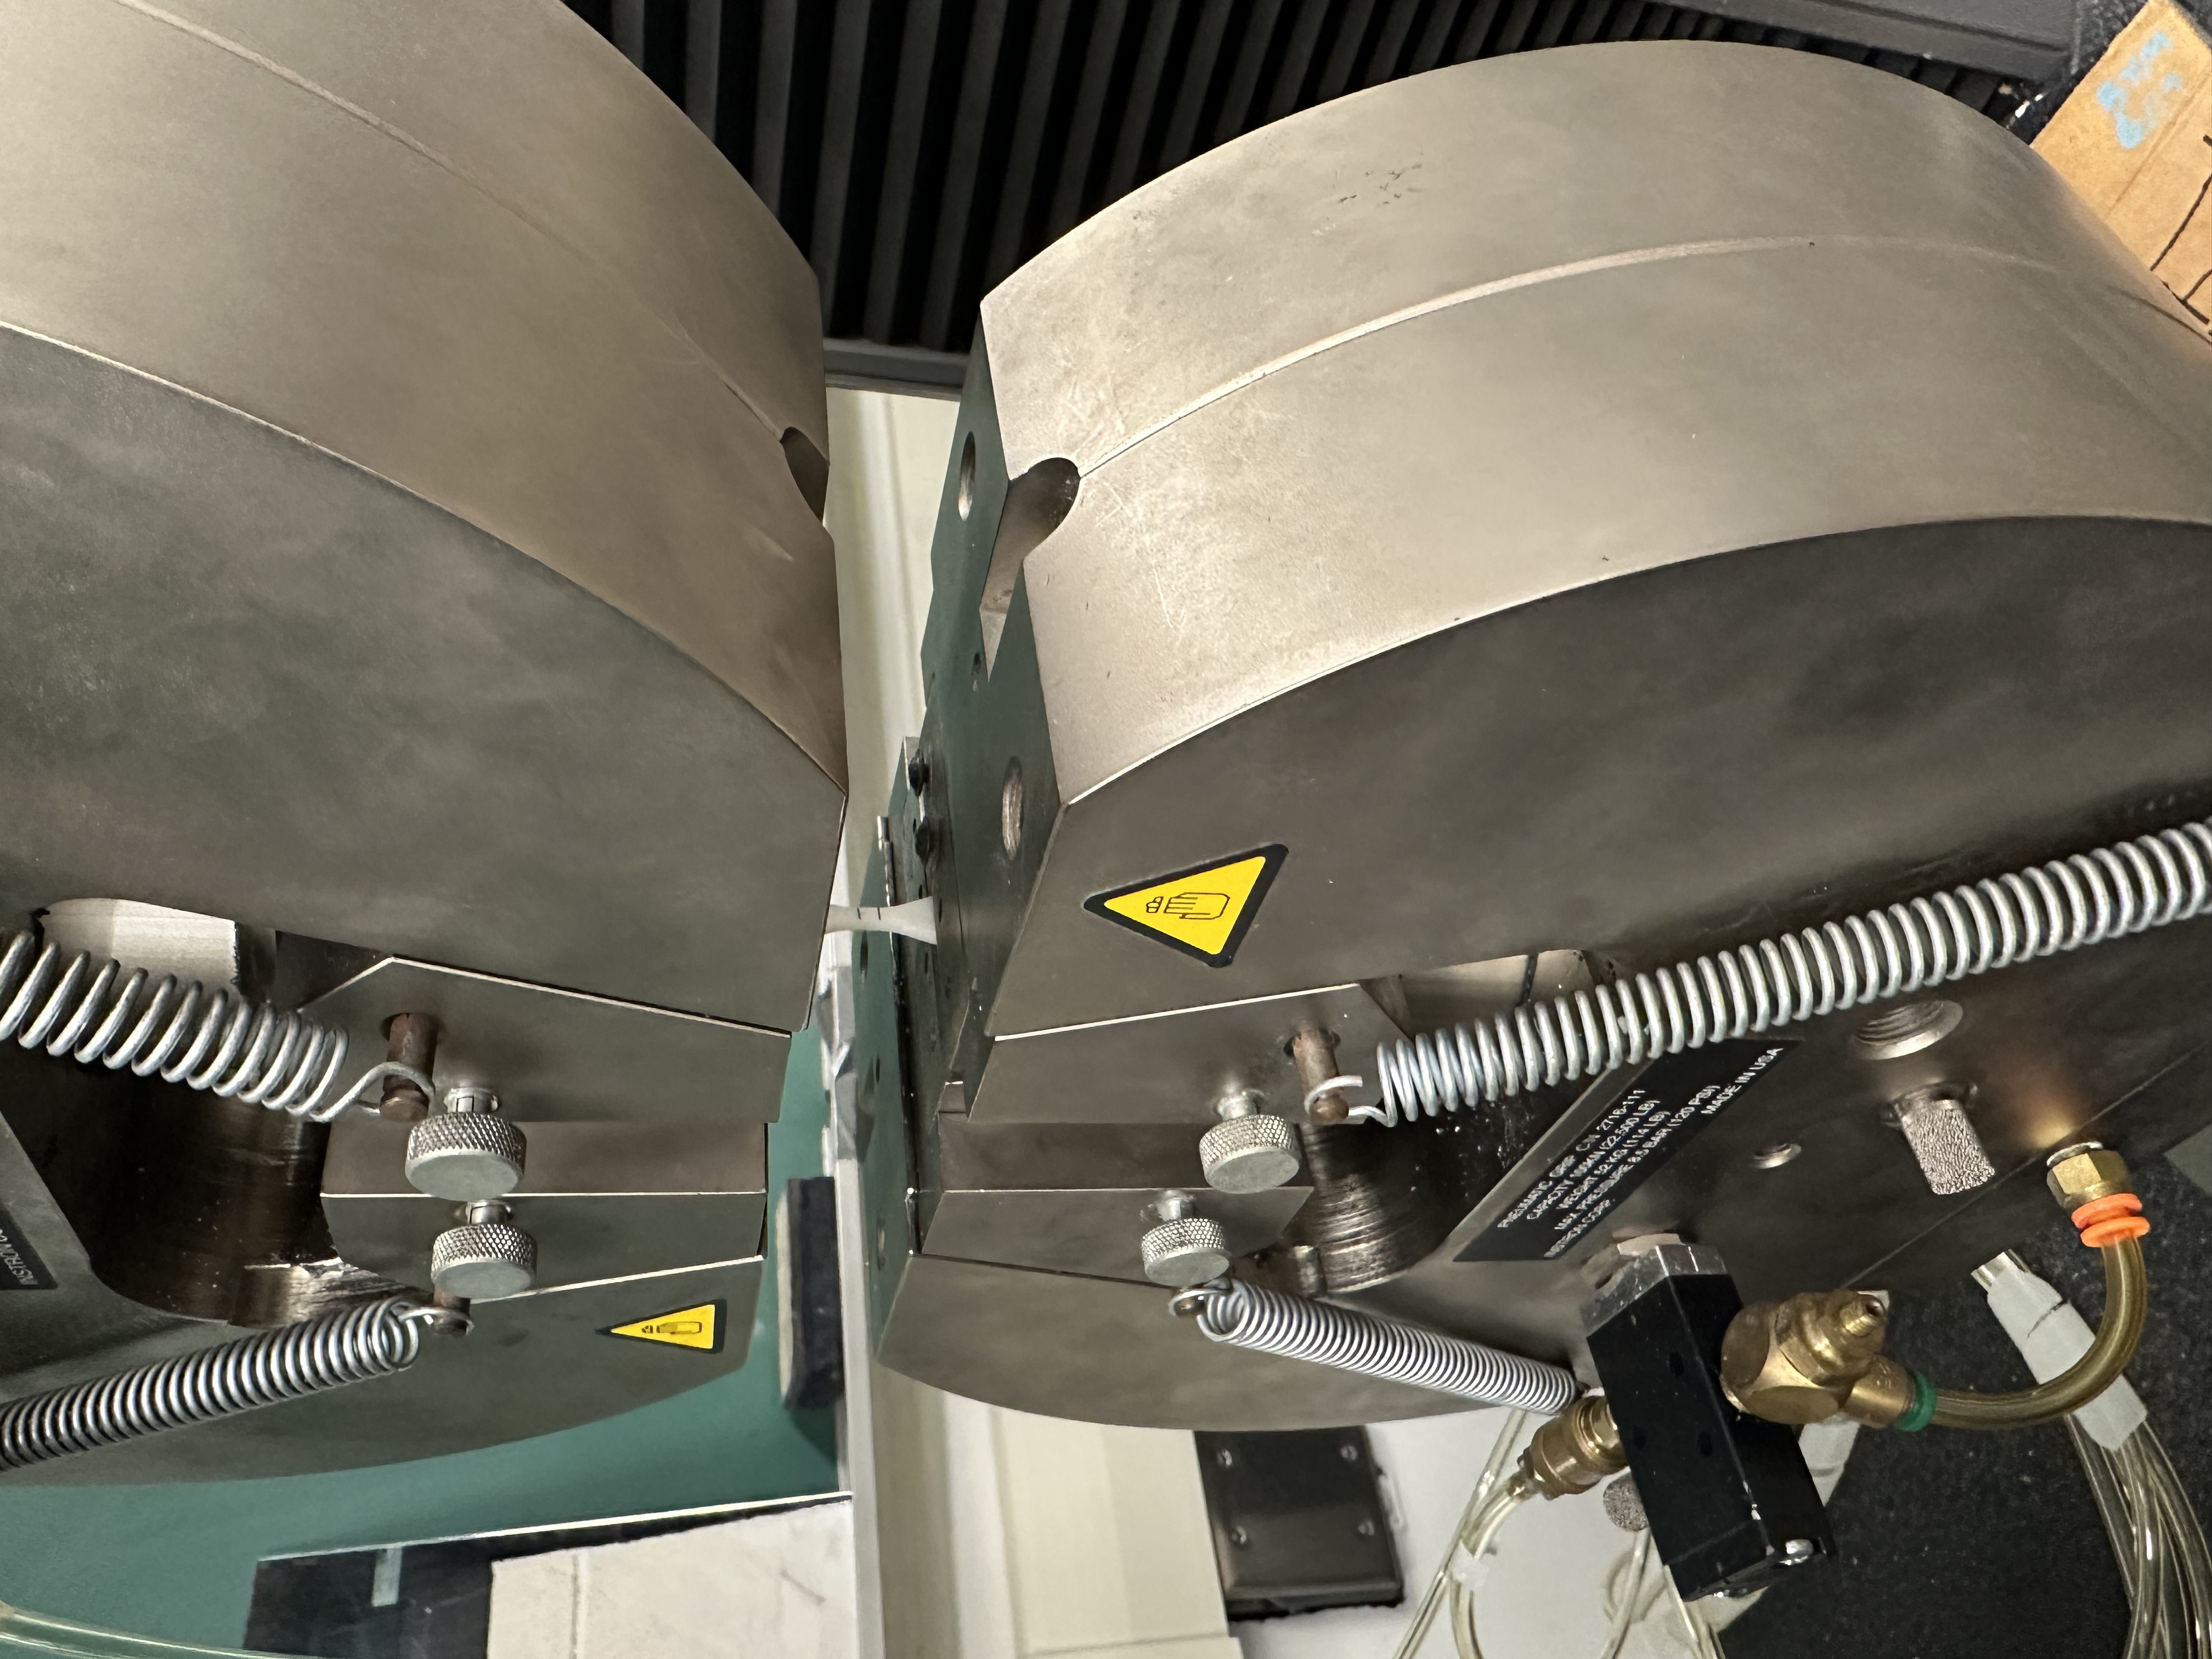
\includegraphics[width=0.5\linewidth]{../figs/methodology/mechanicalTesting/tensileTesting/loaded_sample.png}
        \caption{Sample loaded into Instron for tensile testing.}
        \label{fig:methodology:effectsofBaSO4:tensileTest:loadingSamples}
\end{figure}

\subsubsection{Tensile Test Calculations\label{sec:methodology:effectsOfBaSO4:tensileTesting:calculations}}

\paragraph*{Tensile Strength at Yield}

The yield strength is calculated by dividing the maximum load sustained by the specimen by the initial cross-sectional area as shown in Equation~\eqref{eq:tensileStrength}~\cite{RefWorks:RefID:4-test}. $\sigma_y$ is the yield strength in $MPa$, $F_{max}$ is the maximum applied force, and $A_C$ is the original cross-sectional area of the test specimen.

\begin{equation}
        \sigma_y (MPa) = \frac{F_{max}}{A_C}
        \label{eq:tensileStrength}
\end{equation}

\paragraph*{Elastic Modulus}

The elastic modulus is calculated by taking the slope of the linear portion of the stress vs strain curve. This curve is calculated automatically through Instron software.

Results and discussion of the Type V tensile testing can be found in~\fullref{sec:results:effectsOfBaSO4:tensileTesting:typeV} and~\fullref{sec:discussion:effectsOfBaSO4:tensileTesting:typeV} respectively.

\subsubsection{Type IV Specimen Testing\label{sec:methodology:effectsOfBaSO4:tensileTesting:typeIVSpecimens}}

Due to the unexpected results of the Type V specimen testing and the inability to calculate elastic modulus, Type IV test specimens were 3D printed. The procedure was identical to the testing using Type V test specimens. This time, however, a strain gauge was attached during the tensile test to record strain and create a stress vs strain curve.

Because Type IV specimens are more regularly used than Type V specimens, a template existed to easily mark and measure the dimensions of the test specimen. The sample preparation and test setup are shown below in Figure~\ref{fig:methodology:effectsOfBaSO4:tensileTesting:typeIV}.

\begin{figure}[h!]
        \centering
        \includegraphics[width=0.5\linewidth]{../figs/methodology/mechanicalTesting/tensileTesting/type_iv_tensile_testing.png}
        \caption{Running a tensile test with Type IV specimens. Sample preparation (A) and test setup (B).}
        \label{fig:methodology:effectsOfBaSO4:tensileTesting:typeIV}
\end{figure}

Results and discussion of the Type IV tensile testing can be found in~\fullref{sec:results:effectsOfBaSO4:tensileTesting:typeIV} and~\fullref{sec:discussion:effectsOfBaSO4:tensileTesting:typeIV} respectively.

\subsection{Flexural Testing\label{sec:methodology:effectsOfBaSO4:flexuralTesting}}

Flexural testing was performed to measure the flexural modulus of each PLA/BaSO\textsubscript{4} filament. The flexural modulus shows how a material bends or deflects under a load. It was found that barium sulfate can increase the stiffness of a material. Flexural testing was performed to verify and determine the maximum amount of barium sulfate that can be incorporated without making the implant too stiff for use.

All flexural testing was performed using a Mark-10 Universal Test Machine at CDME.

\subsubsection{Sample Preparation\label{sec:methodology:effectsOfBaSO4:flexuralTesting:samplePrep}}

Samples were prepared following ASTM D790 test standard. Following this standard, rectangular test specimens $12.7mm$ wide, $3.2mm$ thick, and $127mm$ long were 3D printed.

\subsubsection{Performing Flexural Test}

First, measurements of test specimens were taken and recorded. The support span was calculated with a 16:1 support span-to-depth ratio.

The rate of crosshead motion was calculated using Equation~\eqref{eq:flexuralCrossheadMotion}. R is the rate of motion ($mm/min$), L is the support span ($mm$), d is the depth of the beam ($mm$), and Z is the rate of straining of the outer fiber which is set equal to 0.01.

\begin{equation}
        R = \frac{ZL^2}{6d}
        \label{eq:flexuralCrossheadMotion}
\end{equation}

Next, the maximum allowable midspan deflection was calculated using Equation~\eqref{eq:flexuralMaxDeflection}. D is the midspan deflection ($mm$), r is the strain which is set to 0.05$mm/mm$, L is the support span ($mm$), and d is the depth of the beam ($mm$).

\begin{equation}
        D = \frac{rL^2}{6d}
        \label{eq:flexuralMaxDeflection}
\end{equation}

Using these equations, Table~\ref{tab:methodology:effectsOfBaSO4:flexuralTesting:sampleMeasurements} summarizes the measurements and calculated values for all samples.

\begin{table}[h!]
        \centering
        \caption{Measurements and calculated values for flexural testing.}
        \label{tab:methodology:effectsOfBaSO4:flexuralTesting:sampleMeasurements}
        \begin{adjustbox}{width=\textwidth}
                \begin{tabular}{c l l c c c c c c}
                        \hline
                        \textbf{Test \#} & \textbf{Sample Group} & \textbf{Material} & \textbf{D (Avg)} & \textbf{W (Avg)} & \textbf{Full Length (Avg)} & \textbf{Support Span} & \textbf{Rate R} & \textbf{Deflection at 0.05 Strain} \\
                        \hline
                        1                & 0\% BaSO$_4$          & PLA               & 3.350            & 12.617           & 126.553                    & 53.600                & 1.429           & 7.147                              \\
                        2                & 0\% BaSO$_4$          & PLA               & 3.347            & 12.647           & 126.627                    & 53.547                & 1.428           & 7.140                              \\
                        3                & 0\% BaSO$_4$          & PLA               & 3.350            & 12.697           & 126.747                    & 53.600                & 1.429           & 7.147                              \\
                        4                & 0\% BaSO$_4$          & PLA               & 3.347            & 12.690           & 126.667                    & 53.547                & 1.428           & 7.140                              \\
                        5                & 0\% BaSO$_4$          & PLA               & 3.353            & 12.647           & 126.717                    & 53.653                & 1.431           & 7.154                              \\
                        6                & 5\% BaSO$_4$          & PLA               & 3.417            & 12.647           & 126.627                    & 54.667                & 1.458           & 7.289                              \\
                        7                & 5\% BaSO$_4$          & PLA               & 3.480            & 12.693           & 126.640                    & 55.680                & 1.485           & 7.424                              \\
                        8                & 5\% BaSO$_4$          & PLA               & 3.477            & 12.707           & 126.740                    & 55.627                & 1.483           & 7.417                              \\
                        9                & 5\% BaSO$_4$          & PLA               & 3.367            & 12.600           & 126.633                    & 53.867                & 1.436           & 7.182                              \\
                        10               & 5\% BaSO$_4$          & PLA               & 3.363            & 12.627           & 126.660                    & 53.813                & 1.435           & 7.175                              \\
                        11               & 10\% BaSO$_4$         & PLA               & 3.363            & 12.640           & 126.673                    & 53.813                & 1.435           & 7.175                              \\
                        12               & 10\% BaSO$_4$         & PLA               & 3.363            & 12.643           & 126.713                    & 53.813                & 1.435           & 7.175                              \\
                        13               & 10\% BaSO$_4$         & PLA               & 3.370            & 12.663           & 126.470                    & 53.920                & 1.438           & 7.189                              \\
                        14               & 10\% BaSO$_4$         & PLA               & 3.353            & 12.540           & 126.643                    & 53.653                & 1.431           & 7.154                              \\
                        15               & 10\% BaSO$_4$         & PLA               & 3.393            & 12.627           & 126.627                    & 54.293                & 1.448           & 7.239                              \\
                        \hline
                \end{tabular}
        \end{adjustbox}
\end{table}

Results and discussion of the flexural testing can be found in~\fullref{sec:results:effectsOfBaSO4:flexuralTesting} and~\fullref{sec:discussion:effectsOfBaSO4:flexuralTesting} respectively.
